% Options for packages loaded elsewhere
\PassOptionsToPackage{unicode}{hyperref}
\PassOptionsToPackage{hyphens}{url}
%
\documentclass[
  a4paper,
]{article}
\usepackage{amsmath,amssymb}
\usepackage{setspace}
\usepackage{iftex}
\ifPDFTeX
  \usepackage[T1]{fontenc}
  \usepackage[utf8]{inputenc}
  \usepackage{textcomp} % provide euro and other symbols
\else % if luatex or xetex
  \usepackage{unicode-math} % this also loads fontspec
  \defaultfontfeatures{Scale=MatchLowercase}
  \defaultfontfeatures[\rmfamily]{Ligatures=TeX,Scale=1}
\fi
\usepackage{lmodern}
\ifPDFTeX\else
  % xetex/luatex font selection
\fi
% Use upquote if available, for straight quotes in verbatim environments
\IfFileExists{upquote.sty}{\usepackage{upquote}}{}
\IfFileExists{microtype.sty}{% use microtype if available
  \usepackage[]{microtype}
  \UseMicrotypeSet[protrusion]{basicmath} % disable protrusion for tt fonts
}{}
\makeatletter
\@ifundefined{KOMAClassName}{% if non-KOMA class
  \IfFileExists{parskip.sty}{%
    \usepackage{parskip}
  }{% else
    \setlength{\parindent}{0pt}
    \setlength{\parskip}{6pt plus 2pt minus 1pt}}
}{% if KOMA class
  \KOMAoptions{parskip=half}}
\makeatother
\usepackage{xcolor}
\usepackage[margin=1in]{geometry}
\usepackage{longtable,booktabs,array}
\usepackage{calc} % for calculating minipage widths
% Correct order of tables after \paragraph or \subparagraph
\usepackage{etoolbox}
\makeatletter
\patchcmd\longtable{\par}{\if@noskipsec\mbox{}\fi\par}{}{}
\makeatother
% Allow footnotes in longtable head/foot
\IfFileExists{footnotehyper.sty}{\usepackage{footnotehyper}}{\usepackage{footnote}}
\makesavenoteenv{longtable}
\usepackage{graphicx}
\makeatletter
\def\maxwidth{\ifdim\Gin@nat@width>\linewidth\linewidth\else\Gin@nat@width\fi}
\def\maxheight{\ifdim\Gin@nat@height>\textheight\textheight\else\Gin@nat@height\fi}
\makeatother
% Scale images if necessary, so that they will not overflow the page
% margins by default, and it is still possible to overwrite the defaults
% using explicit options in \includegraphics[width, height, ...]{}
\setkeys{Gin}{width=\maxwidth,height=\maxheight,keepaspectratio}
% Set default figure placement to htbp
\makeatletter
\def\fps@figure{htbp}
\makeatother
\setlength{\emergencystretch}{3em} % prevent overfull lines
\providecommand{\tightlist}{%
  \setlength{\itemsep}{0pt}\setlength{\parskip}{0pt}}
\setcounter{secnumdepth}{-\maxdimen} % remove section numbering
\ifLuaTeX
\usepackage[bidi=basic]{babel}
\else
\usepackage[bidi=default]{babel}
\fi
\babelprovide[main,import]{catalan}
% get rid of language-specific shorthands (see #6817):
\let\LanguageShortHands\languageshorthands
\def\languageshorthands#1{}
\ifLuaTeX
  \usepackage{selnolig}  % disable illegal ligatures
\fi
\usepackage{bookmark}
\IfFileExists{xurl.sty}{\usepackage{xurl}}{} % add URL line breaks if available
\urlstyle{same}
\hypersetup{
  pdftitle={U3. WINDOWS SERVER. ADMINISTRACIÓ I CONFIGURACIÓ},
  pdfauthor={@tofermos 2024},
  pdflang={ca-ES},
  hidelinks,
  pdfcreator={LaTeX via pandoc}}

\title{U3. WINDOWS SERVER. ADMINISTRACIÓ I CONFIGURACIÓ}
\author{@tofermos 2024}
\date{}

\begin{document}
\maketitle

{
\setcounter{tocdepth}{2}
\tableofcontents
}
\setstretch{1.5}
\newpage
\renewcommand\tablename{Tabla}

\section{1 Funcions d'un servidor}\label{funcions-dun-servidor}

Des del punt de vista del que series les funcions d'un Sisteam Operatiu
de Xarxa trobem, com ja hem vist a l'anterior unitat, que es corresponen
a alguns dels Rols i Característiques. Podem dir que Windows Server les
implementa així. No tots els Rols i Característiques, menys encara, són
funcions principals.

\begin{enumerate}
\def\labelenumi{\arabic{enumi}.}
\item
  La funció de Servei de Directori que a Linux serà en OpenLDAP i vorem
  més avant, ací els el \textbf{Active Directory Domain Services (AD
  DS)}: Permet crear i gestionar dominis de forma centralitzada i
  còmoda.
\item
  La funció o servei de \textbf{DHCP Server}: Assigna automàticament
  adreces IP als dispositius de la xarxa.
\item
  \textbf{DNS Server}: Traduïx noms de domini a adreces IP, facilitant
  l'accés als serveis dins d'una xarxa o a internet. Convé que recordeu
  que quan cofiguràvem les IP en un WorkGroup NO indicàvem cap IP de
  servidor DNS. En canvi si buscàvem per la xarxa el nom del PC que
  compartia una carpeta, el trobàvem. En un Domini, usem la ressolució
  de noms, molt més eficient.
\item
  \textbf{File and Storage Services}: Gestiona el sistema
  d'emmagatzematge de fitxers i carpetes compartides, i permet utilitzar
  el servidor de fitxers, les quotes d'emmagatzematge i la deduplicació
  de dades.
\item
  La connexió remota pot considerar-se com una funció dels servidors.
  \textbf{Remote Desktop Services (RDS)} Proporciona eines per permetre
  que els usuaris es connecten de forma remota a escriptoris virtuals o
  aplicacions publicades.
\item
  \textbf{Print and Document Services}: Permet gestionar impressores i
  compartir-les en la xarxa.
\item
  \textbf{Web Server (IIS)}: Hosteja aplicacions web i llocs web
  utilitzant \textbf{Internet Information Services (IIS)}.
\item
  \textbf{Servici de backup de Seguretat de Windows Server}. El vorem.
\end{enumerate}

\section{2 Administració i configuració
bàsica}\label{administraciuxf3-i-configuraciuxf3-buxe0sica}

\subsection{Consoles i altres utilitats comuns a tots el sistemes
Windows}\label{consoles-i-altres-utilitats-comuns-a-tots-el-sistemes-windows}

Al curs de Windows 11 d'aquest repositori podreu trobar una guia més que
suficient sobre les utitlitas gràfiques del sistema Windows per
configurar i administrar una màquina.

\href{https://tofermos.github.io/Windows11/gestiodelequip/gestiodelequip.html}{Consoles
i altres utilitats}

\subsection{Consoles i altres utilitats específiques de Windows
Server}\label{consoles-i-altres-utilitats-especuxedfiques-de-windows-server}

A banda de les vistes en l'apartat anterior i que són comunes, la
pràctica totalitat, a tots els Windows tenim que, específicament de
Windows Server les consoles i utilitats següents:

\textbf{servermanager.exe} - Administrador de Servidors. Aquesta és la
utilitat (no es consola estrictament parlant) central per a gestionar el
servidor. Permet configurar rols i característiques, gestionar discos,
supervisar el rendiment, entre altres funcions.

\textbf{dcpromo.msc} - Promoció de controlador de domini: Utilitzada per
configurar un controlador de domini (AD DS), una funció exclusiva de
Windows Server.

\textbf{dnsmgmt.msc} - Gestió de DNS: Disponible en Windows Server per
gestionar zones i registres DNS.

\textbf{dhcpmgmt.msc} - Gestió de DHCP: Permet administrar el rol de
servidor DHCP per assignar adreces IP automàticament a dispositius de la
xarxa.

\textbf{fsmgmt.msc} - Carpetes compartides: Una consola específica per
gestionar carpetes i recursos compartits al servidor, encara que també
es pot trobar en versions professionals de Windows 10/11.

\emph{(els 2 següents no anem a mirar-los en SOX)}

\textbf{tsadmin.msc} o Remote Desktop Services Manager: Utilitzada per
gestionar sessions d'escriptori remot, més comuna en Windows Server per
administrar entorns d'escriptori remot (RDS).

\textbf{cluadmin.msc} - Gestió de Clúster de Failover: Disponible en
Windows Server per administrar clústers de tolerància a fallades i alta
disponibilitat, especialment útil per entorns crítics empresarials.

\subsection{PowerShell (El vorem més
avant)}\label{powershell-el-vorem-muxe9s-avant}

Més avant, si farem una ullada interessant al lleguatge d'scripts basat
en cmdLets (comandaments de Windows) molt avaçat i potent.

Si voleu consultar, teniu un curs de PowerShell en aquest repositori:

\href{https://github.com/tofermos/PowerShell}{Curs PowerShell}

\section{3 Administració i configuració de comptes
locals}\label{administraciuxf3-i-configuraciuxf3-de-comptes-locals}

Els comptes locals perden importància en un Domini. No obstant podeu
consultar el curs de Windows 1x d'aquest repositori, ja que és un tema
comú a tots els Windows Server.

\href{https://tofermos.github.io/Windows11/gestions/comptesLocals.html}{Comptes
locals}

\section{4 Servei de directori}\label{servei-de-directori}

\subsection{4.1 Conceptes de Directori i
Domini}\label{conceptes-de-directori-i-domini}

Bàsicament podem entendre un directori com una llista detallada
d'objectes. Per exemple, l'agenda de tlf del mòbil és un tipus de
directori que guarda informació de contactes de persones o entitats.
Objectes per igual (contactes) que poden tindre nom, adreça, tlf,
e-mail, malnom\ldots{}

\subsubsection{Dos classes
d'informació}\label{dos-classes-dinformaciuxf3}

L'Active Directory Domain Services (AD DS) és molt semblant però més
flexible i dinàmic. Permet emmagatzemar la informació de tota
l'organització. Una informació sobre l'estructura de l'propi directori i
també sobre com s'ha d'administrar. AD DS pot emmagatzemar informació
sobre l'organització, llocs, ordinadors, usuaris, objectes compartits i
qualsevol altra cosa que pugui formar part de la infraestructura de
xarxa. A diferència de la llista de contactes de whatsapp, ací els
elements emmagatzemats son de diferent naturales (usuaris, grups, UO,
polítiques d'accés, permisos, assignació de recursos, etc.) Cal recordar
que tota aquesta informació s'emmagatzema en una base de dades
jeràrquica.

\subsubsection{Replicable}\label{replicable}

El motor d'aquesta base de dades és el mateix que incorpora Microsoft
Exchange Server i permet la replicació de controladors de domini. És a
dir, es pot enviar la informació continguda a la base de dades a
diferents controladors de domini a través de la xarxa.

A més d'administrar polítiques que seran vàlides a tota l'organització,
Active Directory permet realitzar operacions com la instal·lació de
programes, de manera simultània i centralitzada, en multitud de clients
o aplicar actualitzacions crítiques en tota l'organització.

Quan utilitzem Active Directory, tenim a la nostra disposició eines
d'administració per establir polítiques de grup, per incloure uns grups
dins d'altres en diferents nivells, un accés senzill a l'arbre
d'usuaris, ordinadors, impressores i contactes, etc. Òbviament, podem
utilitzar Windows Server 2019 sense usar Active Directory, però estarem
prescindint d'un ampli conjunt de capacitats.

\subsubsection{Dos tipus de components}\label{dos-tipus-de-components}

Pel que fa a l'estructura de l'servei de directori, el primer que hem de
saber és que hi ha dos tipus de components en Active Directory: els
components físics i els components lògics.

\emph{Taula 1: Components de l'AD-DS}

\begin{longtable}[]{@{}ll@{}}
\toprule\noalign{}
Components físics & Components lògics \\
\midrule\noalign{}
\endhead
\bottomrule\noalign{}
\endlastfoot
Controladors de dominis & Dominis \\
Llocs & Boscos \\
Xarxes & Arbres \\
& Unitats organitzatives \\
\end{longtable}

\begin{quote}
Nota:

Al mòdul de SOX ens centrem en desenvolupar un model senzill
d'organització: un Domini amb Unitats Organitzatives.
\end{quote}

\subsection{4.2 Instal·lació del Active
Directory}\label{installaciuxf3-del-active-directory}

Teniu una guia molt resumida en el curs de Windows Server d'aquest
repositori. Entreu al següent enllaç\ldots{}

\href{https://github.com/tofermos/Windows-Server/blob/main/md/ADDSenWindowsServerGUI.md}{Instal·lació
del AD}

\subsection{4.3 Usuaris del Domini}\label{usuaris-del-domini}

A la present unitat i en avant, anem a centrar-nos en els usuaris del
domini. Sobre usuaris locals (els que usem en monoestació o WorkGroup)
teniu tota la informació al curs de Windows 1x d'aquest repositori.

Recordem que els grups són un tipus de contenidor que permeten definir
conjunts d'usuaris i definir permisos basant-nos en aquesta pertinença
al grup, en lloc de fer-ho de manera individual, usuari per usuari. Com
a pauta general, l'agrupació d'objectes sol facilitar les tasques
d'administració reduint les possibilitats d'error.

\subsubsection{Creació d'usuaris}\label{creaciuxf3-dusuaris}

Tot i que després vorem com poden ser els usuaris, és a dir a quin o
quins grups poden pertànyer, fem una mirada prèvia al manteniment dels
usuaris per donar un enfoc pràctic i més dinàmic.

\subsubsection{Des de l'Adminsitrador de l'Active
Directory}\label{des-de-ladminsitrador-de-lactive-directory}

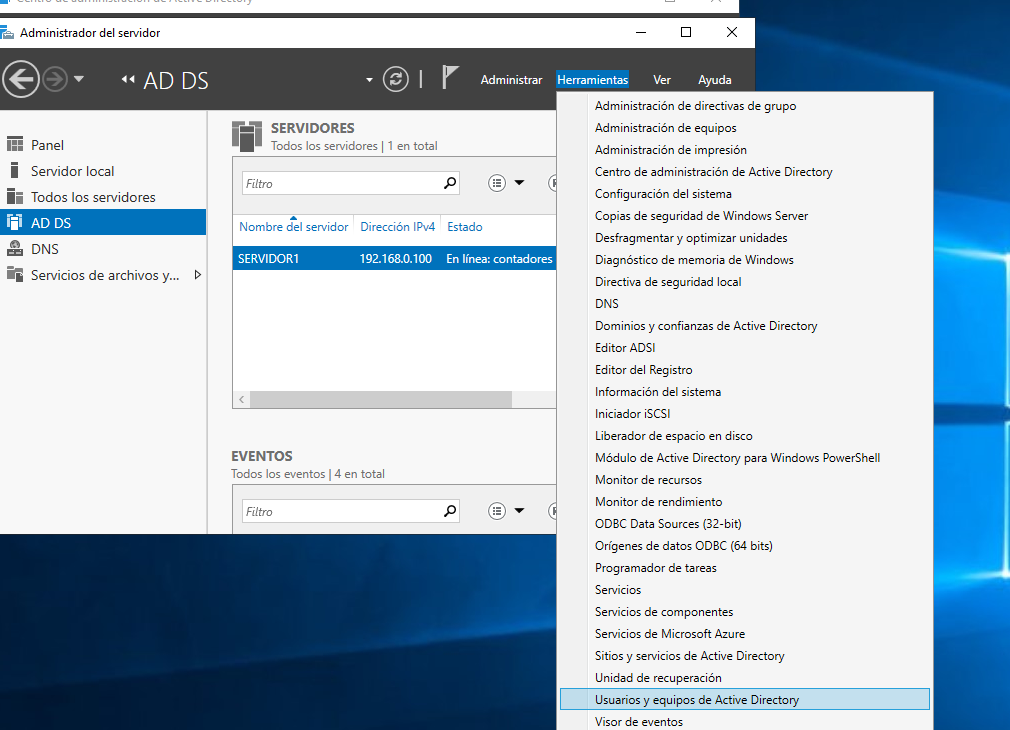
\includegraphics{png/usuaris1.png}

\subsubsection{Creem un usuari}\label{creem-un-usuari}

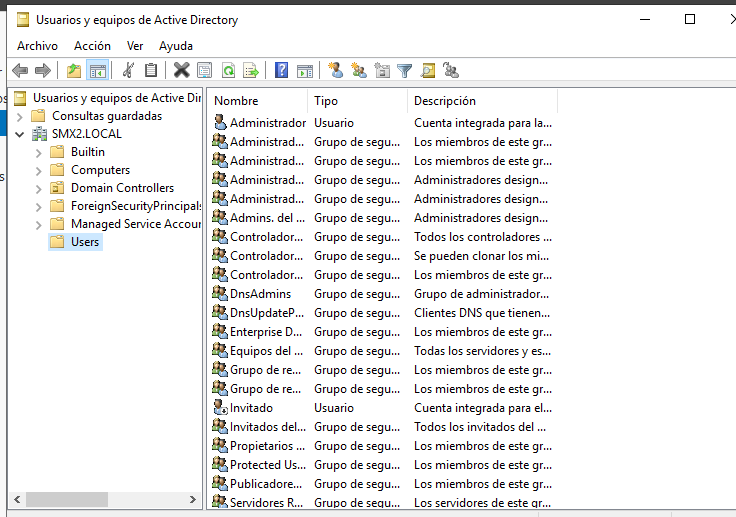
\includegraphics{png/usuaris2.png}

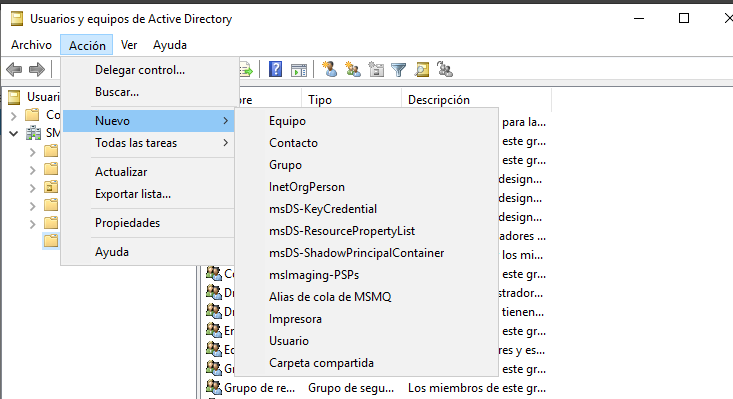
\includegraphics{png/usuaris3.png}

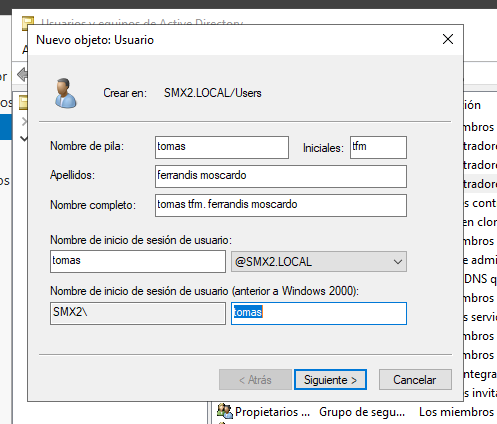
\includegraphics{png/usuaris4.png}

\subsubsection{Configurem el compte d'usuari
creat}\label{configurem-el-compte-dusuari-creat}

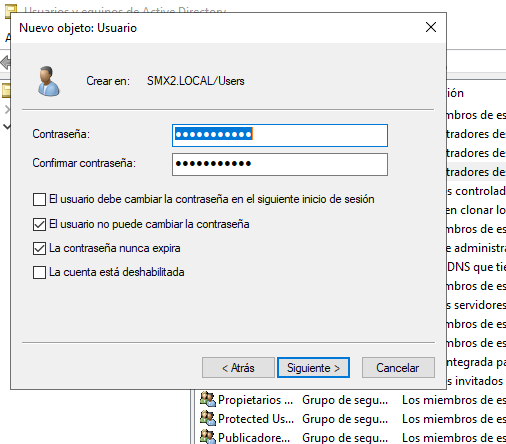
\includegraphics{png/usuaris5.png}

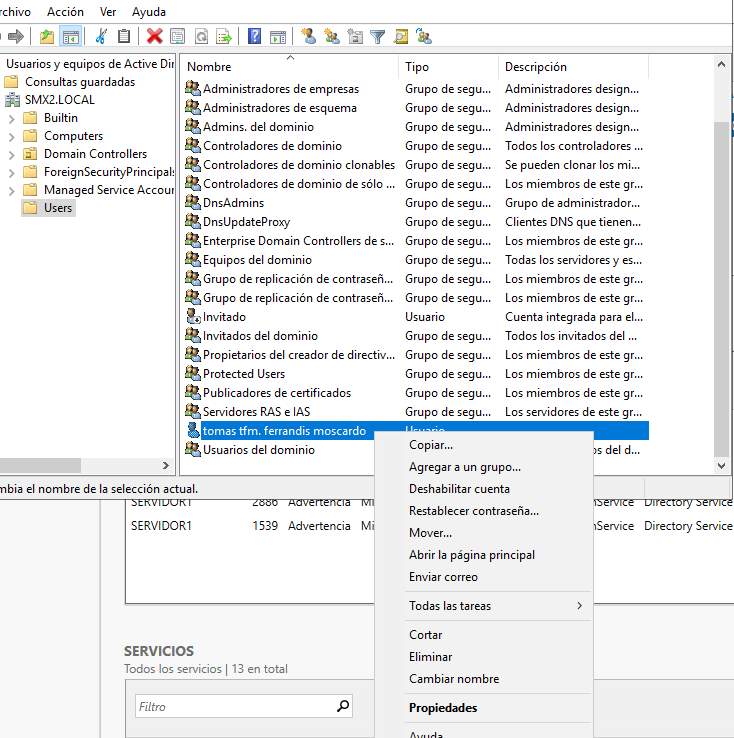
\includegraphics{png/usuaris6.png}

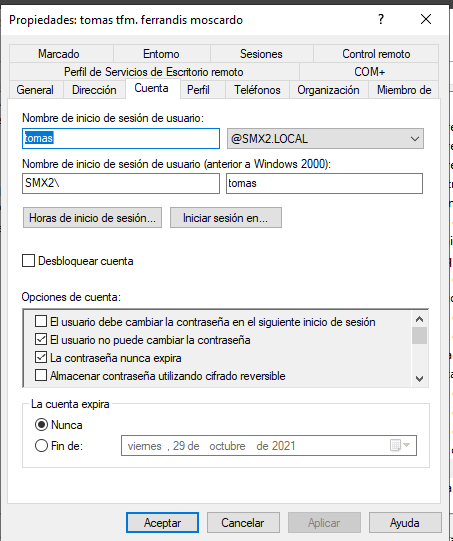
\includegraphics{png/usuaris7.png}

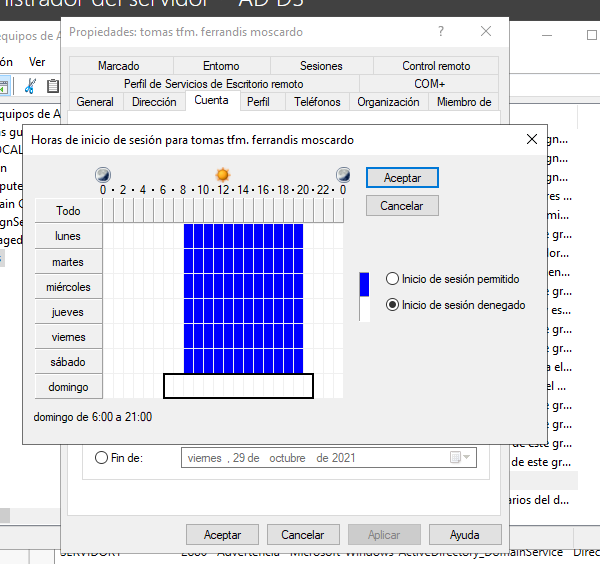
\includegraphics{png/usuaris8.png}

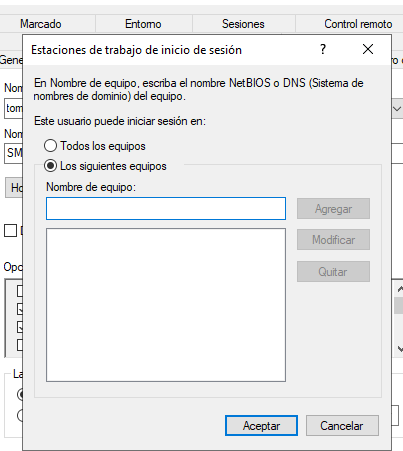
\includegraphics{png/usuaris9.png}

\subsection{4.4 Grups d'usuaris en l'AD}\label{grups-dusuaris-en-lad}

\subsubsection{Tipus i àmbits}\label{tipus-i-uxe0mbits}

Hi ha dos grans tipus de grups al Directori Actiu del Windows:

\textbf{Grups de seguretat:} aquest tipus de grups permet definir
permisos per a recursos del domini. Són els utilitzats a les llistes de
control d'accessos (ACLs) que s'estudiaran més endavant. Aquest tipus de
grups són els que s'utilitzaran a la administració de la xarxa.

\textbf{Grups de distribució:} no tenen característiques de seguretat,
únicament són un llistat d'usuaris per a missatgeria.

Dins dels grups de seguretat hi ha tres àmbits:

\textbf{Grup Universal:} és un grup els permisos del qual s'estenen a
diversos dominis. A més, aquest tipus de grups pot estar format per
usuaris o grups d'usuaris de diferents dominis.

\textbf{Grup Global:} és molt similar als grups universals, és a dir
poden permetre l'accés a recursos de qualsevol dels dominis de l'arbre
del Directori Actiu, però llevat que tots els membres del grup deuen
pertànyer al mateix domini.

\textbf{Grup local del domini:} és un grup creat en un domini amb
membres que poden provenir d'altres dominis i que només pot tenir accés
a recursos dins del domini.

\textbf{En quins casos utilitzarem cada àmbit?}

Els grups universals solen tenir la seva utilitat en grans empreses on
s'ha definit un bosc de dominis assignant dominis a cadascun dels seus
departaments o divisions. En aquest tipus d'estructures, quan se'n
realitza una modificació en el grup, aquesta ha de replicar-se en tots
els controladors de domini que estiguin configurats com a catàleg
global. En xarxes de domini únic es poden aplicar grups globals que
tindran més sentit quan es defineixi un segon domini, el que pot passar
en el moment en què hi hagi una ampliació de l'organització.

Com a pautes generals per a l'administració de xarxes tindrem en compte
les consideracions següents

\begin{enumerate}
\def\labelenumi{\arabic{enumi}.}
\item
  No cal assignar un àmbit més ampli del necessari.
\item
  Els grups locals de domini no es poden processar a altres dominis.
\item
  Un grup global no es replica fora del domini, ja que no forma part del
  pla de replicació del catàleg global.
\item
  Els grups universals es repliquen per tota la xarxa generant trànsit
  que tenia certa incidència en el rendiment abans dels Windows Server
  2008. hui en dia en té poca.
\item
  Si un grup universal està compost per grups globals i es produeixen
  canvis dins dels grups globals, no es produeix un canvi al catàleg
  global, i per tant aquesta modificació no comporta una replicació en
  tots els controladors de domini del bosc.
\end{enumerate}

\subsubsection{Grups predefinits}\label{grups-predefinits}

En instal·lar el Directori Actiu podem comprovar que s'han generat
automàticament una sèrie de grups predefinits amb uns permisos d'acord
amb les funcions assignades:

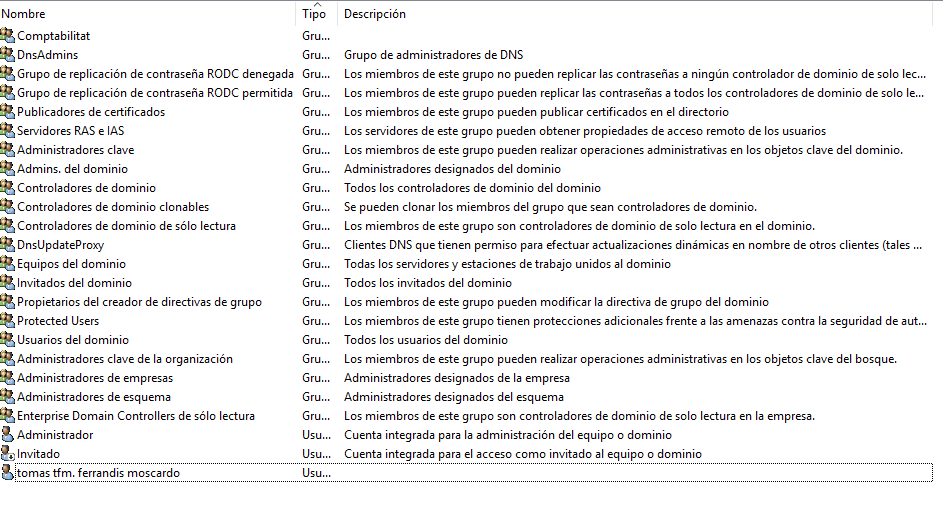
\includegraphics{png/usuaris10.png}

Examinem les funcions d'alguns dels grups més utilitzats:

\textbf{Usuaris del domini:} grup global que conté tots els comptes
d'usuaris del domini.

\textbf{Administradors del domini:} grup global que permet als membres
realitzar tasques d'administració del domini.

\textbf{Administradors d'empresa:} grup universal que permet als membres
realitzar tasques d'administració a tots els dominis de la xarxa.

\textbf{Administradors d'esquema:} grup universal que permet als membres
modificar l'estructura dels objectes del Directori actiu.

\textbf{Administradors:} grup local que permet als seus membres
realitzar tasques d'administració al controlador de domini. Operadors de
còpies de seguretat: grup local que permet als seus membres fer còpies
de seguretat o restaurar fitxers dins del domini.

\textbf{Operadors de compte:} grup local que permet als membres crear,
editar i eliminar comptes d'usuari i grups.

\textbf{Operadors d'impressió:} grup local que permet als membres
configurar i administrar l'ús d'impressores de xarxa.

\textbf{Operadors de servidor:} grup local que permet als seus membres
crear carpetes compartides al servidor i realitzar còpies de seguretat o
restaurar fitxers al controlador de domini.

\textbf{Usuaris:} grup local que limita les possibilitats que un usuari
faci un canvi accidental al sistema però sí permet executar la majoria
de les aplicacions.

\subsubsection{Creació de grups.}\label{creaciuxf3-de-grups.}

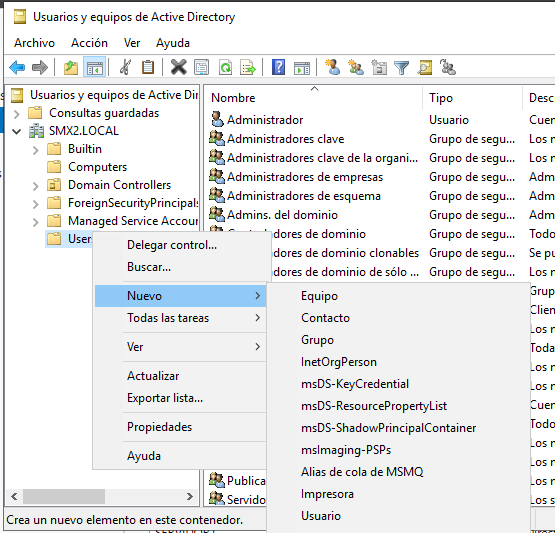
\includegraphics{png/usuaris11.png}

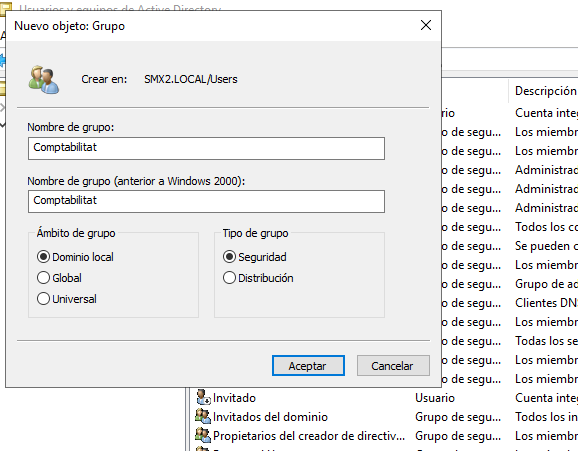
\includegraphics{png/usuaris12.png}

\subsubsection{Com afegir usuaris al
grup.}\label{com-afegir-usuaris-al-grup.}

Opció 1: Propietats del grup\ldots{}

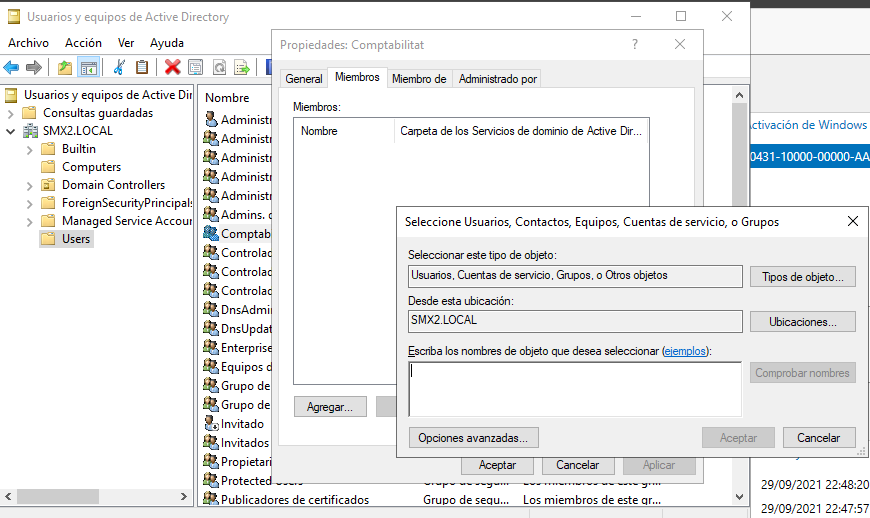
\includegraphics{png/usuaris13.png}

Opció 2: Des de les Propietats de l'usuari\ldots{}

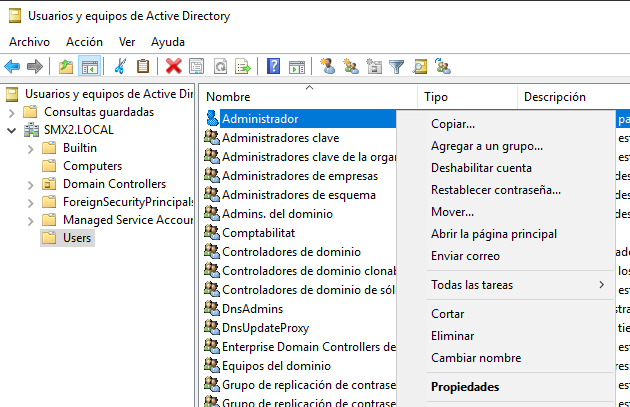
\includegraphics{png/usuaris14.png}

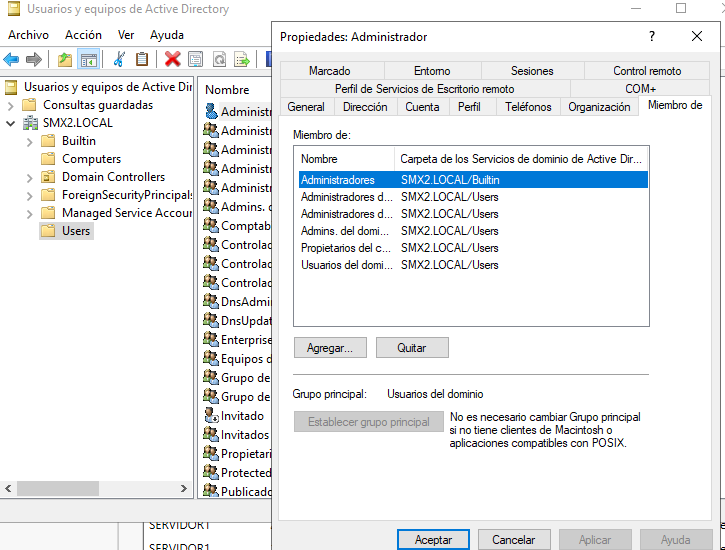
\includegraphics{png/usuaris15.png}

\subsection{4.5 Unitats organitzatives}\label{unitats-organitzatives}

Teniu una guia resumida en el curs de Windows Server d'aquest
repositori. Entreu al següent enllaç\ldots{}

\href{https://github.com/tofermos/Windows-Server/blob/main/md/UnitºatsOrganitzatives.md}{Curs
Windows Server. Unitats Organitzatives}

\section{5 Servei DNS}\label{servei-dns}

L'objecte del mòdul no és l'estudi dels serveis sinó dels Sistemes
Operatius. En aquest cas la integració del servei DNS amb el Windows
Server.

Aquests punt s'aboradarà des de 3 punts de vista:

\begin{itemize}
\tightlist
\item
  Un enfoc teòric en aquest apartat
\item
  Vorem, més avant, alguns cmdLets per instal·lar/desinstal·lar,
  consultar i fer algun canvi.
\end{itemize}

\subsection{5.1 La integració del DNS al servei AD
DS}\label{la-integraciuxf3-del-dns-al-servei-ad-ds}

El servei de servidor DNS està integrat en el disseny i implementació
dels serveis de domini d'Active Directory (AD DS), proporcionant una
eina empresarial per organitzar, gestionar i localitzar recursos en una
xarxa.

Quan implementeu servidors DNS amb AD DS, tingueu en compte que:

\begin{itemize}
\tightlist
\item
  El DNS és necessari per localitzar els controladors de domini.
\item
  El servei d'inici de sessió a la xarxa utilitza el servidor DNS per
  registrar els controladors de domini al vostre espai de noms DNS.
\item
  Els servidors DNS amb Windows Server poden utilitzar AD DS per
  emmagatzemar i replicar les zones DNS.
\item
  La integració de zones DNS amb AD DS permet funcions com la rèplica
  d'AD DS, actualitzacions dinàmiques segures, i l'envelliment i
  eliminació de registres.
\end{itemize}

\textbf{Com s'integra DNS amb AD DS}

Quan instal·leu AD DS en un servidor i el promocioneu a controlador de
domini, se us demana que especifiqueu un nom de domini DNS per al domini
AD DS. A més, se us ofereix l'opció d'instal·lar el servidor DNS, ja que
és necessari per localitzar controladors de domini dins del domini AD
DS.

\subsection{5.2 Beneficis de la integració d'AD
DS}\label{beneficis-de-la-integraciuxf3-dad-ds}

Per a xarxes que utilitzen DNS per a AD DS, es recomana utilitzar zones
primàries integrades al directori, ja que aporten diversos beneficis:

\begin{itemize}
\tightlist
\item
  \textbf{Replicació multimaster}: Amb AD DS, qualsevol servidor DNS pot
  acceptar actualitzacions dinàmiques i replicar-les entre tots els
  servidors DNS.
\item
  \textbf{Seguretat millorada}: Mitjançant ACLs, es poden restringir les
  actualitzacions dinàmiques per a equips o grups específics, cosa que
  no és possible amb zones primàries estàndard.
\item
  \textbf{Automatització i sincronització}: Quan es crea un nou
  controlador de domini, les zones es repliquen automàticament.
\item
  \textbf{Millor rendiment}: La sincronització de les zones integrades
  al directori és més eficient que les actualitzacions estàndard,
  evitant la transferència de tota la zona.
\end{itemize}

Si integreu les zones DNS amb AD DS, també simplifiqueu la gestió de la
rèplica de bases de dades, evitant la necessitat de mantenir topologies
de rèplica separades per a DNS i AD DS. Aquesta integració permet
visualitzar la gestió com una única entitat administrativa.

Finalment, només les zones primàries es poden emmagatzemar al directori.
Les zones secundàries han d'emmagatzemar-se en fitxers de text
estàndard, però amb el model de replicació multimaster d'AD DS, no són
necessàries si totes les zones estan en AD DS.

\section{6 Servei de DHCP}\label{servei-de-dhcp}

El servei \textbf{DHCP (Dynamic Host Configuration Protocol)} en
\textbf{Windows Server} és una funció que permet als administradors de
xarxa automatitzar l'assignació d'adreces IP i altres paràmetres de
configuració de xarxa als dispositius que es connecten a la xarxa.

\subsection{6.1 Funcionament del servei
DHCP}\label{funcionament-del-servei-dhcp}

Es tracta d'un típic servici que respon a la filosofia del model client
servidor. Quan un dispositiu (com un ordinador, càmera IP, mòbil,
impressora\ldots) es connecta a la xarxa, envia una sol·licitud per
obtenir una adreça IP. El servidor DHCP respon a aquesta petició
assignant-li una adreça IP de manera automàtica i dinàmica, així com
altres paràmetres de configuració de xarxa com:

\begin{itemize}
\tightlist
\item
  \textbf{Adreça IP}: Una adreça única dins del rang establit pel
  servidor.
\item
  \textbf{Màscara de subxarxa}: Indica la porció de la xarxa a la qual
  pertany l'adreça IP.
\item
  \textbf{Passarel·la predeterminada}: Normalment, és l'adreça del
  router o un altre dispositiu de xarxa que connecta la xarxa local amb
  Internet.
\item
  \textbf{Servidors DNS}: Les adreces dels servidors que resolen els
  noms de domini a adreces IP.
\end{itemize}

\subsection{6.2 Avantatges del servei DHCP en Windows
Server}\label{avantatges-del-servei-dhcp-en-windows-server}

\begin{itemize}
\tightlist
\item
  \textbf{Gestió centralitzada}: DHCP facilita la gestió de les adreces
  IP des d'un servidor central, evitant la configuració manual de cada
  dispositiu.
\item
  \textbf{Eficàcia}: Assegura que no es produeixin conflictes d'adreces
  IP duplicades a la xarxa.
\item
  \textbf{Escalabilitat}: És especialment útil en xarxes grans, on
  assignar IPs manualment seria lent i poc pràctic.
\item
  \textbf{Flexibilitat}: Si volem un canvi de totes les IP o gran part,
  només hem de configurar-lo al servici i reiniciar el dispositius.
  Imaginem, per exmeple, passar de IPv4 de classe C a B per a tota una
  xarxa.
\item
  \textbf{Actualitzacions automàtiques}: El servidor DHCP pot canviar
  les adreces IP dels dispositius a mesura que es connecten i
  desconnecten de la xarxa.
\item
  \textbf{Concessió temporal d'adreces IP}: Les IPs es poden assignar
  amb una duració específica, de manera que quan un dispositiu deixa de
  ser necessari a la xarxa, l'IP es pot reutilitzar.
\end{itemize}

\subsubsection{Components principals del
DHCP}\label{components-principals-del-dhcp}

\begin{itemize}
\item
  \textbf{Rangs o àmbits}: Un conjunt de configuracions que defineixen
  un rang d'adreces IP que es poden assignar als dispositius clients.
\item
  \textbf{Exclusions}: Quan volem que dins del rang alguna IP o grup
  d'IPs (``subrangs'') no s'assignen. Pot ser útil per si volem
  assignar-les de forma fixa a determinats dipositius.
\item
  \textbf{Reserves}: Permeten assignar una IP fixa a un dispositiu en
  particular basat en la seva adreça MAC, assegurant que sempre obtinga
  la mateixa IP.
\item
  \textbf{Opcions DHCP}: Paràmetres addicionals, com ara passarel·les
  (router o gateway) predeterminades o DNS, que el servidor DHCP pot
  proporcionar als dispositius clients.
\end{itemize}

\subsubsection{Funcionament del procés
DHCP}\label{funcionament-del-procuxe9s-dhcp}

\begin{enumerate}
\def\labelenumi{\arabic{enumi}.}
\tightlist
\item
  \textbf{Discover}: El client envia una petició en difusió per trobar
  un servidor DHCP a la xarxa.
\item
  \textbf{Offer}: El servidor DHCP respon oferint una adreça IP.
\item
  \textbf{Request}: El client accepta l'oferta enviant una sol·licitud
  per a l'adreça IP.
\item
  \textbf{Acknowledge}: El servidor DHCP confirma l'assignació de
  l'adreça IP al client.
\end{enumerate}

\begin{figure}
\centering
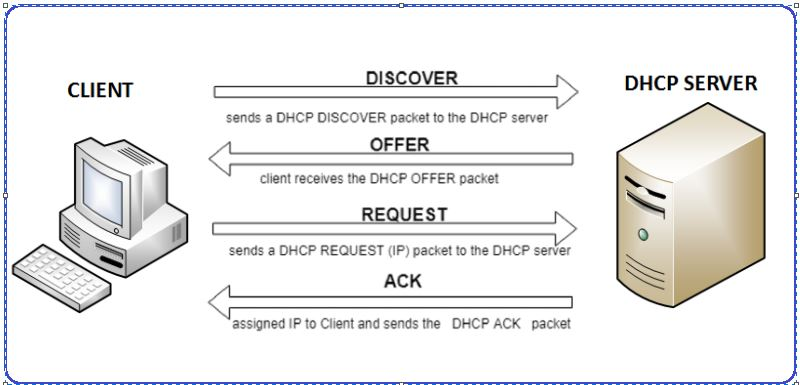
\includegraphics{png/DHCPesquema.jpg}
\caption{\emph{Figura1: Esquema C/S}}
\end{figure}

En resum, el servei DHCP en Windows Server facilita la gestió i
assignació automàtica d'adreces IP en una xarxa, millorant l'eficiència
i reduint la complexitat de la configuració manual de xarxes.

\subsection{6.3 Enfoc pràctic}\label{enfoc-pruxe0ctic}

Aquests punt s'aboradarà des de 3 punts de vista:

\begin{itemize}
\tightlist
\item
  Un enfoc teòric.
\item
  Vorem, més avant, alguns cmdLets per instal·lar/desinstal·lar,
  consultar i fer algun canvi.
\item
  Un enfoc pràctic en usar-los en les activitats desenvolupades des del
  GUI que abordem al següent apartat mitjançant el curs de Windows
  Server d'aquest repositori.
\end{itemize}

\section{6.4 DHCP. Implementación}\label{dhcp.-implementaciuxf3n}

Teniu una guia molt resumida en el curs de Windows Server d'aquest
repositori. Entreu al següent enllaç\ldots{}

\href{https://github.com/tofermos/Windows-Server/blob/main/md/DHCP.md}{}

\end{document}
